\documentclass[12pt]{article}
\usepackage[vmargin=20mm, hmargin=15mm]{geometry} 
\usepackage{multicol}
\usepackage{datetime}
\usepackage{array}
\usepackage{lipsum}
\usepackage{graphicx}
\usepackage{mwe}
\usepackage{tikz-dependency}
\usepackage{float}
\usepackage[normalem]{ulem}
\usepackage[square]{natbib}
  
\geometry{a4paper} 
\frenchspacing
\parindent 0pt
\parskip 6pt
\setlength\columnsep{15pt}

\newcommand{\docvec}{\texttt{doc2vec}}
\newcommand{\wordvec}{\texttt{word2vec}}

%%% BEGIN DOCUMENT
\begin{document}
\centerline{\large NLP Assignment 3 Report}
\vspace{0.1in}
\centerline{\Large\bf Investigating an Automated Question Answering System}
\vspace{0.1in}
\centerline{\large {\bf{Z\'ebulon Goriely, Queens', zg258}}}
\vspace{0.1in}
\centerline{\large {\today}}
%\centerline{\large{Friday 22\textsuperscript{nd} November, 2019}}
\vspace{0.05in}

\makeatletter
\newenvironment{tablehere}
  {\def\@captype{table}}
  {}

\newenvironment{figurehere}
  {\def\@captype{figure}}
  {}
\makeatother

%%% BEGIN BODY OF TEXT
\section*{Introduction}

For all three tasks, I investigated the NLP problem of understanding text. The specific scenario I undertook is the simulation of a second language learner's performance on the IELTS test\footnote{https://www.ielts.org/}. These tests involve reading provided text and answering non-trivial questions, specifically designed to require inference.

Example questions were provided in pdf format, plaintext format and parsed format using the Stanford Parser \citep{chen2014fast} in the framework of a course in NLP.

\section*{Task 1 \\ \small Word Count: 332\footnote{\emph{texcount docs/assignment3/report.tex}}}

The first provided text gives an instruction manual for a Moulex Iron. The first question associated with this text is \emph{``What sort of water are you advised to use?''}. When answering, I implicitly:
\begin{itemize}
  \item Realise that the ``what kind of" question implies that the answer is a subtype of water
  \item Realise that from ``advised to use", the answer is in the context of ``use"
  \item Narrow the answer down to ``distilled water''
\end{itemize}

I can translate this intuition into a hypothetical automated system. To operate on the text and questions, I use dependency parsing \citep{lecture5}. Dependency parsing produces structures that are intuitively closer to the meaning of the text than regular parse trees. It also has the advantage of being neutral to word order.

The hypothetical system restricts answers based on dependencies and begins by analysing the parse and part-of-speech tagging of the question, as seen in Figure \ref{figure:question1}. I then imagine a sub-system that uses this information to derive the question type; the \texttt{WP} tag signifying a ``wh-'' question. The \texttt{nmod:of} and the \texttt{nsubj:xsubj} dependencies in the parse informing the system that answer is a subtype of ``water'' used in the context of ``use''.

The system then compares each occurrence of ``water'' with the parse structures, searching for the dependencies \texttt{compound(water, xx)} or \texttt{amod(water, xx)} and \texttt{dobj(use, water)}. This may involve stemming \citep{lecture2} in order to accept other forms of verbs and nouns. The answer to the question is then \texttt{xx water}.

Figure \ref{figure:sentence2} and Figure \ref{figure:sentence3} show the two solutions that this system finds, ``tap water'' and ``distilled water''. I can use a heuristic to select the second choice, intuitively because detail is likely given later in informative text.

This imaginary system fails, however, when applied to Question 12 of Text 2. Neither the phrasing of the question nor the actual answer (``bathroom'') appear in the text, so a search for \texttt{nmod:for(extra, bathroom)} fails. The inference must be made on the word ``facilities'', indicating the need for a more complex system.

\begin{figure}[H]
\begin{dependency}
   \begin{deptext}[column sep=0.9cm, row sep=.5ex]
      What \& sort \& of \& water \& are \& you \&[.6cm] advised \&[.6cm] to \& use \& ? \\
      WP \& NN \& IN \& NN \& VBP \& PRP \& VBN \& TO \& VB \& .\\
   \end{deptext}
   \deproot[edge unit distance=1cm]{7}{root}
   \depedge{2}{1}{det}
   \depedge{7}{2}{dep}
   \depedge{4}{3}{case}
   \depedge{2}{4}{nmod:of}
   \depedge{7}{5}{auxpass}
   \depedge{7}{6}{nsubjpass}
   \depedge[edge unit distance=0.7cm]{9}{6}{nsubj:xsubj}
   \depedge{9}{8}{mark}
   \depedge{7}{9}{xcomp}
   \depedge{7}{10}{punct}
\end{dependency}
\caption{Stanford parse and part-of-speech tagging of Question 1 from Text 1}
\label{figure:question1}
\end{figure}

\begin{figure}[H]
\begin{dependency}
   \begin{deptext}[column sep=0.9cm]
      Your \& iron \& is \& designed \& to \& function \& using \& tap \& water \& . \\
   \end{deptext}
   \deproot[edge unit distance=1cm]{4}{root}
   \depedge{2}{1}{nmod:poss}
   \depedge{4}{2}{nsubjpass}
   \depedge{6}{2}{nsubj:xsubj}
   \depedge{4}{3}{auxpass}
   \depedge{6}{5}{mark}
   \depedge{4}{6}{xcomp}
   \depedge{6}{7}{xcomp}
   \depedge{9}{8}{\bf{compound}}
   \depedge{7}{9}{\bf{dobj}}
   \depedge{4}{10}{punct}
\end{dependency}
\caption{Stanford parse of Sentence 2 from Text 1 with search-tags in boldface}
\label{figure:sentence2}
\end{figure}

\begin{figure}[H]
\begin{dependency}
   \begin{deptext}[column sep=0.7cm]
      However \& , \& it \& will \& last \& longer \& if \& you \& use \& distilled \& water \&. \\
   \end{deptext}
   \deproot[edge unit distance=1cm]{4}{root}
   \depedge{4}{1}{advmod}
   \depedge{4}{2}{punct}
   \depedge{4}{3}{nsubj}
   \depedge{6}{5}{advmod}
   \depedge{9}{6}{advmod}
   \depedge{9}{7}{mark}
   \depedge{9}{8}{nsubj}
   \depedge{4}{9}{advcl:if}
   \depedge{11}{10}{\bf{amod}}
   \depedge{9}{11}{\bf{dobj}}
   \depedge[edge unit distance=0.4cm]{4}{12}{punct}
\end{dependency}
\caption{Stanford parse of Sentence 3 from Text 1 with search-tags in boldface}
\label{figure:sentence3}
\end{figure}

\vspace{0.5in}

\section*{Task 2 \\ \small Word Count: 332}

I imagine the system attempting to answer the question \emph{``What should you do if your iron starts to drip water?''} for the first text. 

As before, the system uses the dependency parse and part-of-speech tagging of the question (see Figure \ref{figure:question3}) to restrict the possible answers to conform to the dependencies \texttt{dobj(drip ,water)} and \texttt{advcl:if(xx, drip)}. The answer will relate to the verb \texttt{xx}.

Unfortunately, such a verb does not appear in the text. The system can be improved by using lexical semantics \citep{lecture7} to rank potential answers by lexical similarity.

I explore three different metrics for lexical similarity. Firstly, using pre-trained \wordvec~embeddings provided by Google \citep{mikolov2013distributed}, I find that ``droplets'' is the second-most similar word in the text to ``drip'', as seen in Table \ref{table:drip}. Similarly, exploring the synset of ``drip'' using \emph{WordNet} \citep{miller1995wordnet} gives ``drop'' which is found contained in ``droplet''. Note that I use the noun form of ``drip'', since words that are both nouns and verbs can always be modified by changing the tense or voice. Finally, using \emph{ConceptNet} \citep{speer2016conceptnet} relations (see  Figure \ref{figure:concept}) gives another means of deriving that ``droplet'' is one of the closet words in the document to ``drip''. 

Similarly for Question 2, the phrase \emph{``quantity of steam''} does not appear in the text. Performing a \wordvec~search (see Table \ref{table:quantity}) shows that ``amount'' is the most similar word to ``quantity'', telling the system that the answer lies within the sentence containing ``amount of steam''. This is also supported by \emph{WordNet}, the synset for ``quantity'' containing ``amount'' (see Figure \ref{figure:quantity}).

Combining the lexical ranking of ``drip'' with our dependency parsing lets the system derive that the sentence \emph{``If your iron produces droplets of water instead of giving off steam, your temperature control is set too low''} relates to the answer of Question 3. The \texttt{advcl:if(set-20, produces-6)} dependency gives ``set'' as the verb required. Further inference is required, however, to derive that ``temperature control is set too low'' implies that the answer is ``increase temperature'' which I discuss in task 3.

\begin{figure}[H]
\begin{dependency}
   \begin{deptext}[column sep=0.6cm,  row sep=.5ex]
      What \& should \& you \& do \& if \& your \& iron \& starts \& to \& drip \& water \& ? \\
      WP \& MD \& PRP \& VB \& IN \& PRP\$ \& NN \& VBZ \& TO \& VB \& NN \& . \\
   \end{deptext}
   \deproot[edge unit distance=1cm]{4}{root}
   \depedge{4}{1}{dobj}
   \depedge{4}{2}{aux}
   \depedge{4}{3}{nsubj}
   \depedge[edge unit distance=0.4cm]{8}{5}{mark}
   \depedge{7}{6}{nmod:poss}
   \depedge{8}{7}{nsubj}
   \depedge{10}{7}{nsubj:xsubj}
   \depedge{4}{8}{advcl:if}
   \depedge{10}{9}{mark}
   \depedge{8}{10}{xcomp}
   \depedge{10}{11}{dobj}
   \depedge[edge unit distance=0.4cm]{4}{12}{punct}
\end{dependency}
\caption{Stanford parse and part-of-speech tagging of Question 3 from Text 1}
\label{figure:question3}
\end{figure}

\begin{table}
\parbox{.45\linewidth}{
\centering
\begin{tabular}{|c|c|c|c|} 
     \hline
     Word & Similarity\\ [0.5ex] 
     \hline\hline
    ``drip'' & 1.0 \\
     \hline
    ``spray'' & 0.44 \\
     \hline
    \bf{``droplets''} & 0.36 \\
     \hline
    ``distilled'' & 0.33 \\
     \hline
    ``water'' & 0.32 \\
     \hline
    \end{tabular}
    \caption{The 5 closest words in Text 1 to ``drip'' according to \wordvec} \label{table:drip}
}
\hfill
\parbox{.45\linewidth}{
\centering
\begin{tabular}{|c|c|c|c|} 
     \hline
     Word & Similarity\\ [0.5ex] 
     \hline\hline
    ``quantity'' & 1.0 \\
     \hline
    \bf{``amount''} & 0.44 \\
     \hline
    ``intensity'' & 0.28 \\
     \hline
    ``therefore'' & 0.28 \\
     \hline
    ``produced'' & 0.26 \\
     \hline
    \end{tabular}
    \caption{The 5 closest words in Text 1 to ``quantity'' according to \wordvec} \label{table:quantity}
}
\end{table}

\begin{figure*}[t]
    \begin{minipage}{0.49\textwidth}
        \centering
        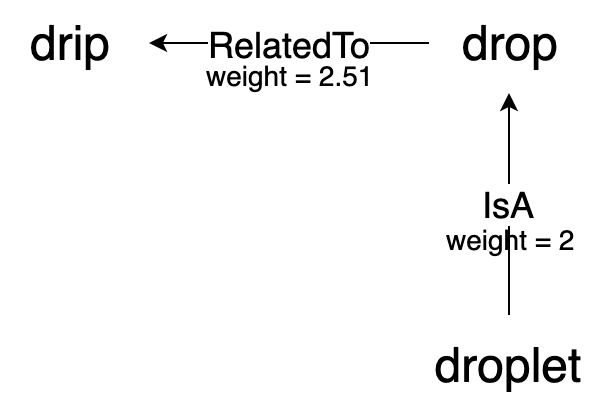
\includegraphics[width=1\textwidth]{figs/concept.png}
        \caption{ConceptNet derivation of ``droplet'' from ``drip''}
        \label{figure:concept}
    \end{minipage}\hfill
    \begin{minipage}{0.49\textwidth}
       \centering
       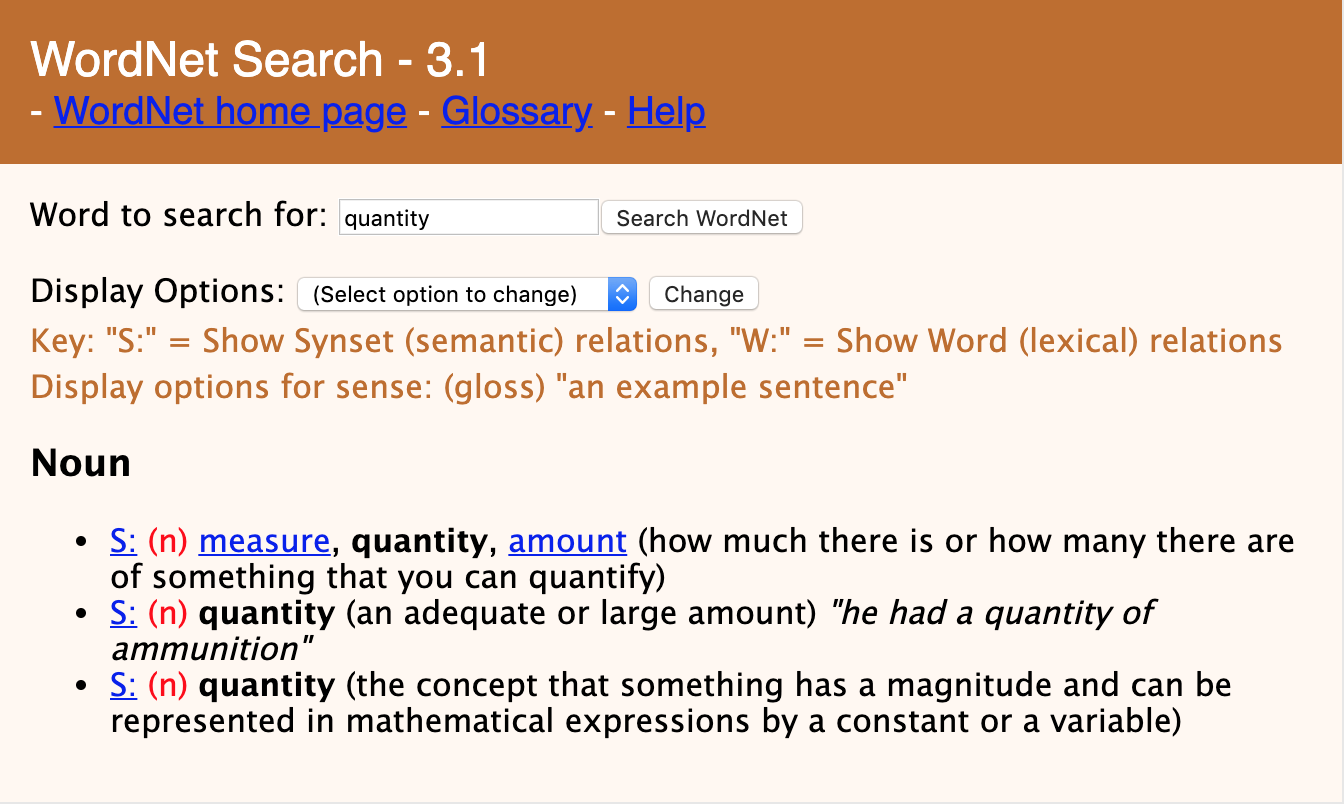
\includegraphics[width=1\textwidth]{figs/synset.png}
       \caption{WordNet search for ``quantity''}
       \label{figure:quantity}
    \end{minipage}
\end{figure*}

\vspace{0.5in}

\section*{Task 3 \\ \small Word Count: 326}

Sometimes, answering questions requires logical reasoning. Question 5 of Text 1 requires the following chain of reasoning:

\begin{itemize}
\item Irons are used to remove creases
\item Do not attempt to remove creases from an item of clothing that is being worn
\item Clothes worn by a person are in direct touch with skin
\item Skin can burn if touched by a hot surface
\item Irons are hot surfaces
\item Burns hurt
\item Ironing clothes being worn can results in a person getting hurt
\end{itemize}

Automating a chain requires inference on a knowledge base \citep{lecture6}. For this task and  other NLP tasks, common sense reasoning a  major obstacle to achieve similar performance to humans. To explore if this automation is possible, I explore how ML is used to solve similar  tasks.

Two popular datasets for the common sense reading comprehension task are the \emph{Story Cloze Test} \citep{mostafazadeh2017lsdsem} and \emph{SemEval-2018 Task 11} \citep{ostermann2018semeval}. Like Question~5, some of the knowledge required to answer the questions may not be found in the documents, requiring systems  to be equipped with some common sense knowledge database. These datasets may be effective for training a system to answer IELTS questions.

Many publicly available knowledge sources already exist, such as \emph{ConceptNet} \citep{speer2016conceptnet}, \emph{WebChild} \citep{tandon2014webchild} and \emph{DeScript} \citep{wanzare2016descript}. 

\citet{wang2018yuanfudao} have shown using \emph{ConceptNet} as a knowledge base can achieve accuracies of 83.95\% on \emph{SemEval-2018 Task 11}, but their system only uses embeddings based on \emph{ConceptNet} as additional input features. They propose that methods based on event calculus \citep{mueller2014commonsense} are more rigorous mathematically and more closely resemble  humans processing.

Performance on these tests has rapidly improved, machine learning models such as in \citep{xia2019incorporating} achieving accuracies of 88.23\% and 87.4\% on \emph{SemEval-2018 Task 11} and \emph{Story Cloze Test} respectively. However, these models make it much more difficult to justify the intermediate steps.

This rapid improvement suggests that achieving an automated system that matches human performance on the IELTS test by 2021 seems possible. Whether or not such systems will be able to justify their answers, as required by the specification, remains to be seen.

\bibliography{refs}
\bibliographystyle{apalike}

\end{document}